\documentclass[11pt]{article}
\usepackage[margin=2.2cm]{geometry}
\usepackage{graphicx,booktabs,amsmath,enumitem,hyperref,xcolor}
\graphicspath{{figures/}}
\setlist{itemsep=2pt,topsep=3pt}
\newcommand{\todo}[1]{\textcolor{red}{\textbf{[TODO: #1]}}}

\title{AI651 -- Deep Learning for Space, Time and Graphs\\Programming Assignment 1}
\author{\todo{Name, Roll number}}
\date{October 2026}

\begin{document}
\maketitle
\noindent\textbf{GitHub repository:} \todo{public repo URL}

\noindent All Task 1 numbers come from the \texttt{PA1\_PRESET=full} run (data seed 0, model seed 0).
Unless stated otherwise, errors are on the \textbf{validation} region (targets in $[9600,12480)$),
in physical units (m/s$^2$), for the population named in each claim.

%=====================================================================
\section*{Task 1 -- Forecasting Across Heterogeneous Sensors}

%---------------------------------------------------------------------
\subsection*{Response 1A -- Predicted vs.\ measured ordering}

\textbf{Prediction (written before running Output 1.1).} \todo{your own predicted ordering for
established stations and for Station 4, written before seeing Output 1.1}

\begin{table}[h]\centering\small
\begin{tabular}{lcccccccc}\toprule
 & \multicolumn{4}{c}{Established (Stations 1--3)} & \multicolumn{4}{c}{Held-out Station 4}\\
\cmidrule(lr){2-5}\cmidrule(lr){6-9}
Model & All & A & B & C & All & A & B & C\\\midrule
Shared ridge          & 0.767 & 0.805 & 0.854 & 0.621 & 0.876 & 0.909 & 0.982 & 0.713\\
Sensor-specific ridge & 0.768 & 0.804 & 0.852 & 0.630 & -- & -- & -- & --\\
Period-routed ridge   & \textbf{0.166} & \textbf{0.181} & \textbf{0.164} & \textbf{0.152} & \textbf{0.173} & \textbf{0.184} & \textbf{0.182} & \textbf{0.150}\\
Raw Attention         & 0.417 & 0.396 & 0.447 & 0.405 & 0.581 & 0.604 & 0.561 & 0.576\\\bottomrule
\end{tabular}
\caption{Output 1.1: validation RMSE (m/s$^2$). Parameters: 4.6k / 13.8k / 59.9k / 368k; fit time
$<$0.05\,s for every ridge vs.\ $\approx$102\,s for Raw Attention.}
\end{table}

\textbf{Measured ordering} (both populations): period-routed ridge $<$ Raw Attention $<$ shared
ridge $\approx$ sensor-specific ridge.
\begin{itemize}
  \item \textbf{Context beats identity.} Sensor-specific ridge is no better than shared ridge
  (0.768 vs.\ 0.767): splitting by station does not remove the pace mixture, because every station
  sees all three products. It also has no model for Station 4.
  \item \textbf{Routing on the right variable wins by a lot.} Period-routed ridge cuts the
  established RMSE by 78\% vs.\ shared ridge (0.767$\to$0.166) and is 2.5$\times$ better than Raw
  Attention, using 6$\times$ fewer parameters and no training loop. Within one 1.5-sample pace
  band the continuation \emph{is} close to a single linear map, so least squares no longer has to
  compromise.
  \item \textbf{Attention learns some context dependence, but not all.} Raw Attention halves the
  shared-ridge error (0.767$\to$0.417) without being told the period, but it has to learn the
  conditioning from data and carry the slow ramp in the same representation.
  \item \textbf{Generalisation gap.} Moving from established stations to Station 4, period-routed
  ridge degrades by only 4\% (0.166$\to$0.173), shared ridge by 14\%, and Raw Attention by 39\%
  (0.417$\to$0.581). The hand-built router depends only on pace, which Station 4 shares; Attention
  partly fits station-specific amplitude/offset/drift patterns.
  \item \textbf{Products.} Ridge baselines are worst on Product B and best on Product C;
  period-routed ridge is flat across products, which again shows that its error no longer depends
  on which pace is active.
\end{itemize}
\textbf{Revision.} \todo{state how your prior ordering changed, e.g.\ ``I expected Raw Attention
to beat every ridge; the hand-routed linear model beat it by 2.5$\times$''}

%---------------------------------------------------------------------
\subsection*{Response 1B -- Why the rule must depend on context}

\begin{figure}[h]\centering
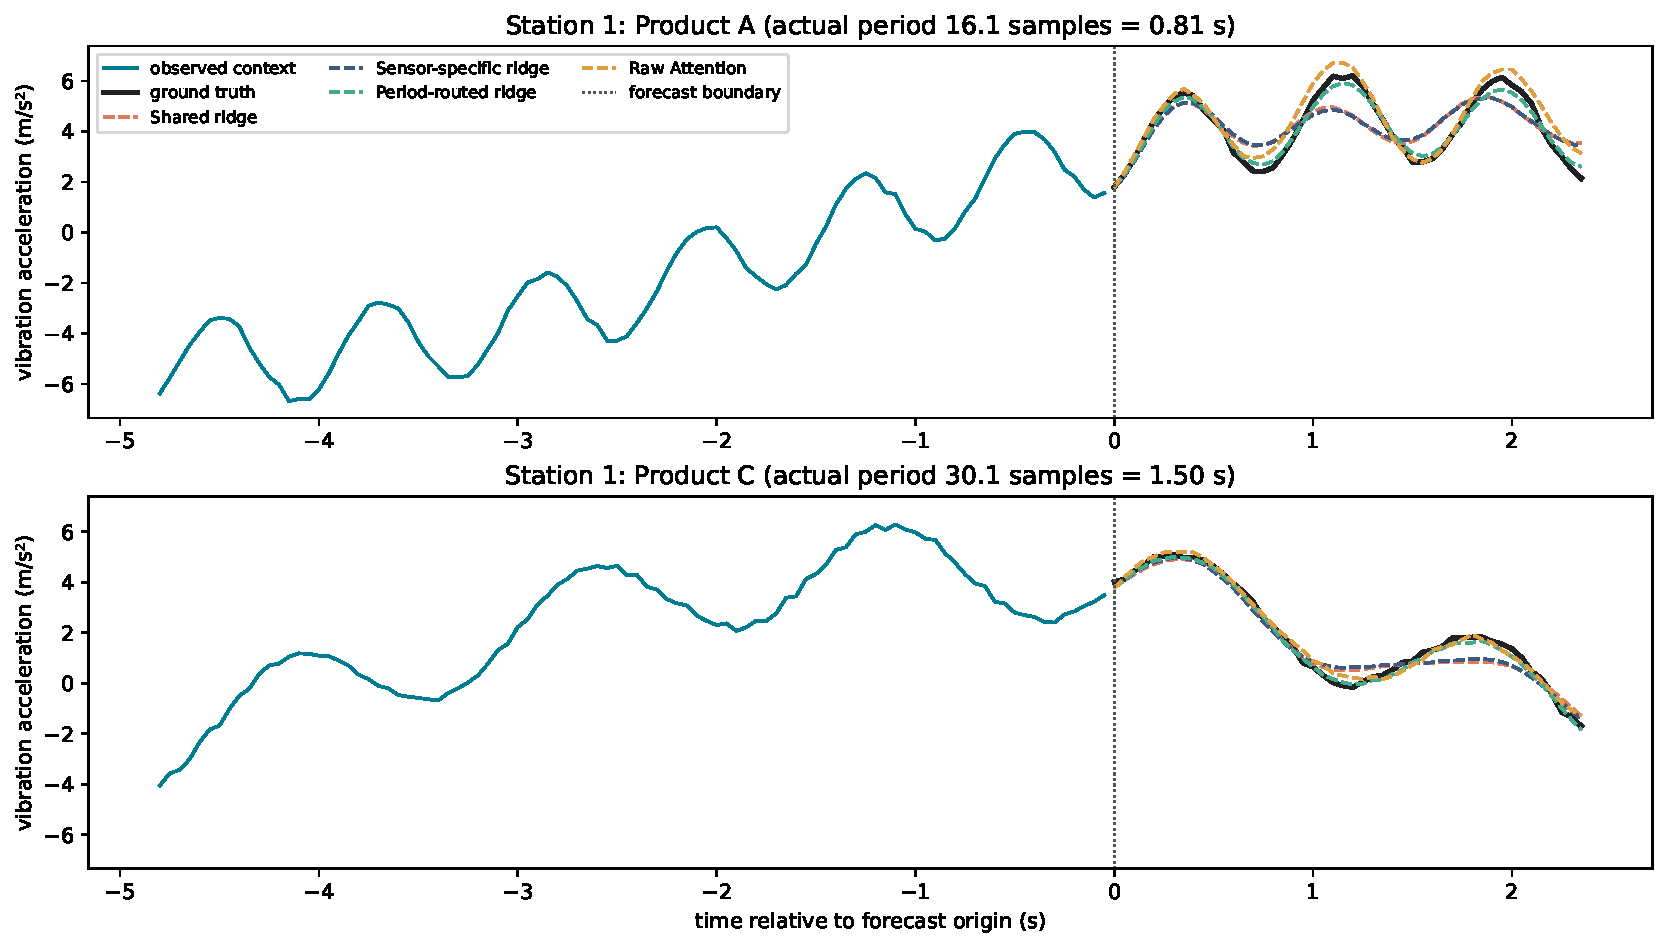
\includegraphics[width=.85\linewidth]{1.2-1.pdf}
\caption{Output 1.2: Station 1, validation; Product A (period 16.1) and Product C (period 30.1).}
\end{figure}

\begin{itemize}
  \item \textbf{The compromise.} $\widehat W$ in Eq.~(8) is fit once over windows whose periods span
  14--36 samples. For one anchored context, the correct next peak lies at a phase advance that
  depends on $P$; a single linear operator cannot choose between these, so least squares returns
  roughly an \emph{average} of the continuations for all paces. Averaging sinusoids with different
  periods produces \textbf{amplitude shrinkage and phase blurring}.
  \item \textbf{Visible in Output 1.2.} For Product A, shared and sensor-specific ridge get the
  first peak roughly right, then flatten: their second and third peaks are about 1\,m/s$^2$ too low
  and their troughs about 1\,m/s$^2$ too high (window RMSE 0.78 vs.\ 0.23 for period-routed ridge).
  For Product C they miss the second trough and peak near 1.5--2\,s (window RMSE 0.45 vs.\ 0.15).
  The error grows with lead time because the phase mismatch accumulates.
  \item \textbf{Attention builds a new operator per context.} $W_Q,W_K,W_V$ are frozen after
  training, but the mixing matrix $\mathrm{softmax}(QK^\top/\sqrt{d_h})$ is a function of the
  current window $X$. In Output 1.3, the same Station 1 projections produce visibly different maps
  for the Product A and Product C contexts: the differences are concentrated near the most recent
  keys, the maximum absolute weight difference is 0.43, and the mean is 0.013. So the
  value-mixing operation, and hence the effective linear map applied to the values, changes with the
  input, while ridge applies the same $\widehat W$ to both.
  \item \textbf{Caveat.} Output 1.3 shows only that the mixing weights depend on context. It is not
  evidence that Attention has recovered the physical period.
\end{itemize}

\begin{figure}[h]\centering
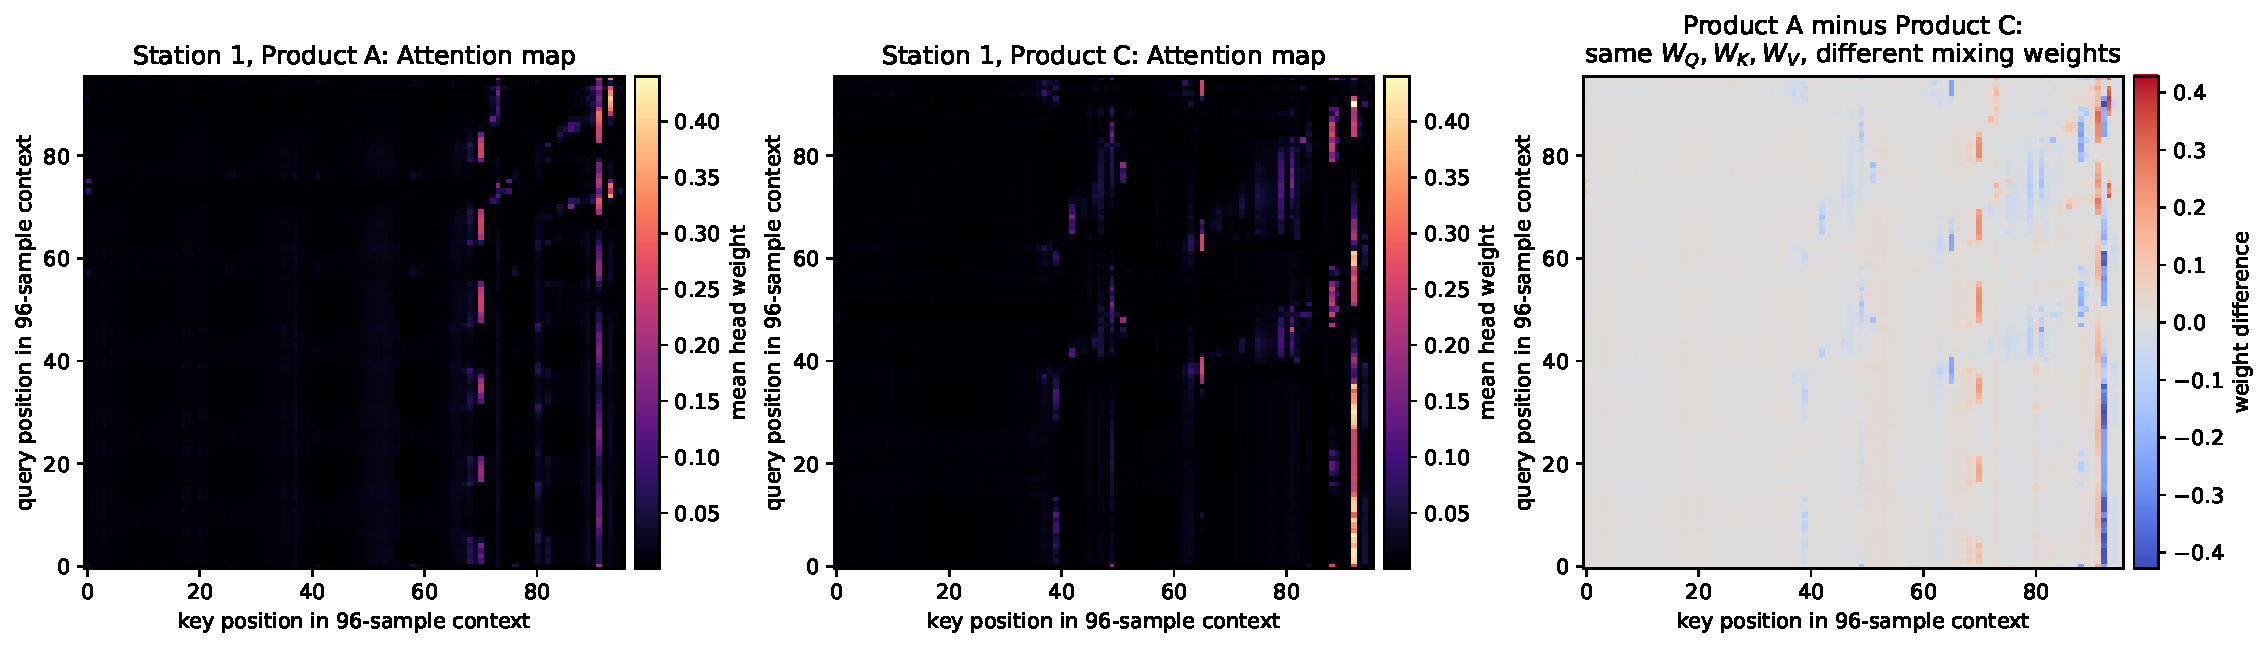
\includegraphics[width=\linewidth]{1.3-1.pdf}
\caption{Output 1.3: Raw Attention maps (mean over heads), Station 1, validation.}
\end{figure}

%---------------------------------------------------------------------
\subsection*{Response 2 -- Separating slow structure from repetition}

\textbf{Selected width: $m=41$.}
\begin{itemize}
  \item \textbf{Visual (Output 2.1, Station 2, Product C, validation).} With narrow widths (17, 25)
  the trend still wiggles with the vibration, so part of the cycle leaks into $T$ and the remainder
  is damped (residual std 0.58\,m/s$^2$ at $m=17$). As $m$ grows the trend becomes a smooth ramp
  and the remainder becomes a full-amplitude, zero-centred oscillation (std 1.57 at $m=41$). The
  projection score at the true period (32) is sharp after decomposition and almost flat on the raw
  context. The endpoints use replicate padding, so the last $\approx$20 samples of $T$ flatten
  towards the final value; this is visible at the right edge of the plot.
  \item \textbf{Oracle diagnostic (Output 2.2, established stations, training region only).}
  Recovery of the true period to within one sample rises from 68.7\% on the raw context to
  98.0 / 98.9 / 99.3 / \textbf{99.8}\% for $m=17/25/33/41$.
  \item \textbf{Ablation (Output 2.3, validation).} Adding decomposition to the same Attention
  forecaster lowers the RMSE for every product and both populations:
  \begin{center}\small
  \begin{tabular}{lcccccc}\toprule
   & \multicolumn{3}{c}{Established} & \multicolumn{3}{c}{Held-out Station 4}\\
   \cmidrule(lr){2-4}\cmidrule(lr){5-7}
   & A & B & C & A & B & C\\\midrule
   Raw Attention & 0.396 & 0.447 & 0.405 & 0.604 & 0.561 & 0.576\\
   Attention + decomposition & \textbf{0.277} & \textbf{0.339} & \textbf{0.288} & \textbf{0.397} & \textbf{0.482} & \textbf{0.466}\\
   Relative change & $-30\%$ & $-24\%$ & $-29\%$ & $-34\%$ & $-14\%$ & $-19\%$\\\bottomrule
  \end{tabular}\end{center}
  It still does not match period-routed ridge (0.15--0.18).
  \item \textbf{Why a moving average is the right bias here.} The world is a slow component
  (240-sample time scale) plus a fast cycle (14--36 samples). A moving average is a low-pass
  filter: with a width at least as long as the vibration period, the cycle averages to roughly zero
  inside the window, while the slow component, which is nearly linear over 41 samples, passes
  through. The trend head can then extrapolate the ramp linearly, and the encoder sees a
  zero-mean repeating signal.
  \item \textbf{Why the oracle diagnostic is a sound way to pick $m$.} The goal of the split is to
  expose the repetition. Period recovery measures that directly, using the generator's known
  period on \emph{training} windows from established stations only, so the validation set,
  Station 4 and the test set do not influence the choice of $m$. The true period is used only for
  scoring, never as a model input.
  \item \textbf{Where it fails or an alternative.} A centered moving average assumes the trend is
  locally linear and changes much more slowly than the width. An abrupt level shift (e.g.\ a
  calibration jump) would be smeared over $m$ samples and leak a step-shaped artefact into $S$.
  \textbf{Alternative:} STL/LOESS or a Fourier low-pass decomposition encodes ``the trend is the
  low-frequency band'' and adapts to curvature better, but it needs a cutoff frequency and is
  costlier to apply inside every block.
\end{itemize}

\begin{figure}[h]\centering
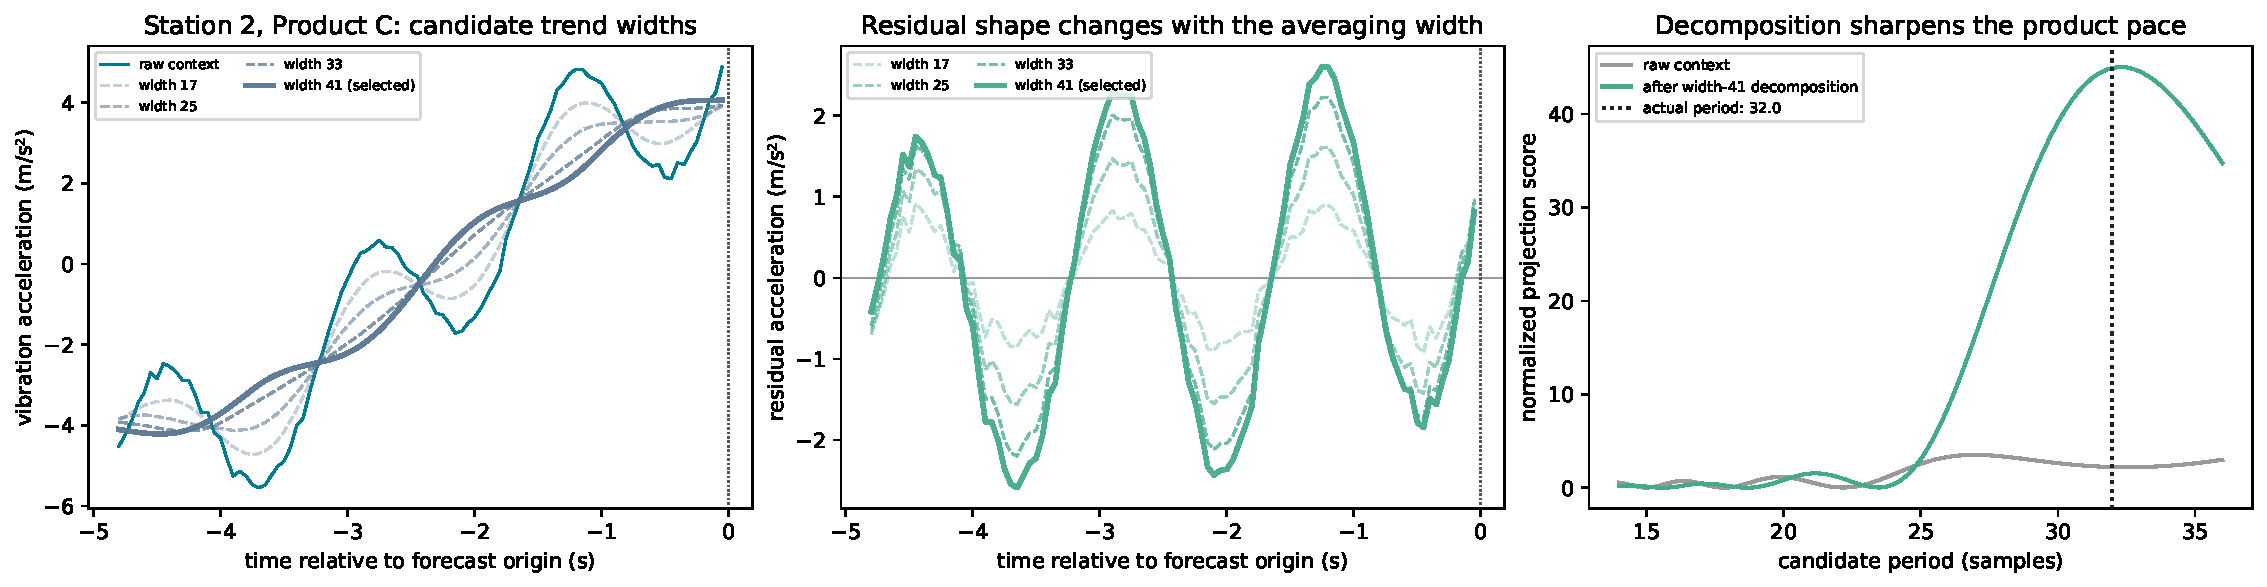
\includegraphics[width=\linewidth]{2.1-1.pdf}
\caption{Output 2.1: candidate widths on one validation context (Station 2, Product C).}
\end{figure}

%---------------------------------------------------------------------
\subsection*{Response 3 -- Mixing by temporal delay}

\texttt{aggregate\_delays} implements Eq.~(6) with a per-example \texttt{gather} on the index
$(t-\tau_j)\bmod L$. The worked example gives $z=[35,15,25,25]$ (so $z_0=35$ and the direction is
correct), and the notebook's value and gradient checks pass. Output 3.1 confirms
\texttt{delay\_scores} on $[1,3,1,3]$: scores $[4,-4,4,-4]$.

\begin{figure}[h]\centering
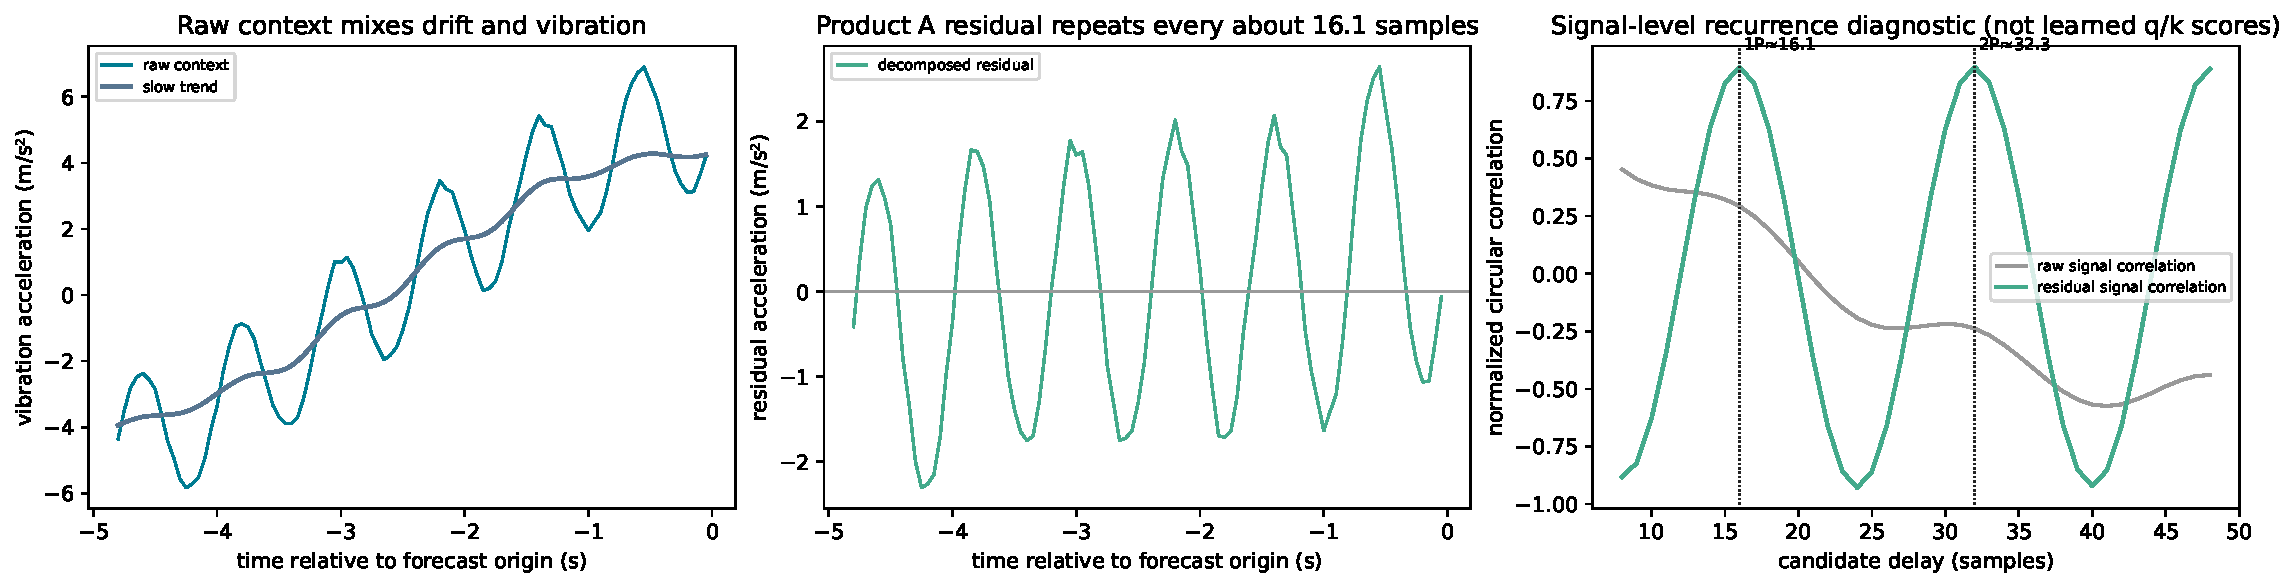
\includegraphics[width=\linewidth]{3.2-1.pdf}
\caption{Output 3.2: signal-level recurrence diagnostic (validation; Station 2, Product A,
$P\approx16.1$). This is a correlation computed directly from the signal, \emph{not} the
model's learned $q/k$ scores.}
\end{figure}

\begin{itemize}
  \item \textbf{Strongest lags.} The residual correlation peaks at delay 16 (0.896) and 32
  (0.897), the nearest integers to $P=16.1$ and $2P=32.3$. It has troughs of about $-0.9$ near
  $P/2\approx 8$, $3P/2\approx24$ and $5P/2\approx40$, and rises again towards $3P\approx48$. The
  recurrence sits on integer multiples of the run's period.
  \item \textbf{Why decomposition cleans the evidence.} The raw-signal correlation simply decays
  from 0.45 to about $-0.55$ across the band and has \emph{no} peak at $P$. A rising ramp
  correlates with itself at every small shift, and circular wrapping joins the high end of the ramp
  to its low start, so the ramp dominates the score. Removing the trend leaves a zero-mean
  oscillation in which aligned peaks add and misaligned ones cancel. The top-$K$ selection then
  picks $P$ and its multiples instead of the smallest delays. This supports the delay mixer's
  assumption: once drift is removed, the useful relationships really are organised by a few
  displacements.
  \item \textbf{When the bias is wrong.} \emph{Isolated transients}, such as a one-off impact
  inside the context: delay aggregation copies values from $t-\tau_j$, so the spike is replayed
  every $\tau_j$ samples into the representation and forecast, producing ``ghost'' echoes of an
  event that will not recur. Similarly, a \emph{period that drifts within the window} (a machine
  spinning up) has no single lag that aligns the whole window, so the correlation peaks smear out
  and the blended shifted copies go out of phase. Pairwise Attention can treat each position on
  its content and does not have this problem.
\end{itemize}

%---------------------------------------------------------------------
\subsection*{Response 4 -- Compare designs and deploy}

\textbf{(a) Prediction (before Output 4.1).} \todo{your own $\le$2-sentence prediction, written
before running Output 4.1}

\textbf{(b) Validation results} (Outputs 4.1--4.2; MSE in (m/s$^2$)$^2$, RMSE in m/s$^2$).
\begin{center}\small
\begin{tabular}{lcccccc}\toprule
 & \multicolumn{2}{c}{Established} & \multicolumn{2}{c}{Held-out St.\,4} & & \\
 \cmidrule(lr){2-3}\cmidrule(lr){4-5}
Model & RMSE & MSE & RMSE & MSE & Params & Fit (s)\\\midrule
Shared ridge              & 0.767 & 0.588 & 0.876 & 0.767 & 4{,}608   & 0.002\\
Sensor-specific ridge     & 0.768 & 0.590 & --    & --    & 13{,}824  & 0.031\\
Period-routed ridge       & \textbf{0.166} & \textbf{0.028} & \textbf{0.173} & \textbf{0.030} & 59{,}904 & 0.004\\
Raw Attention             & 0.417 & 0.174 & 0.581 & 0.338 & 368{,}368 & 101.7\\
Attention + decomposition & 0.302 & 0.091 & 0.450 & 0.202 & 373{,}024 & 188.3\\
Raw delay mixer           & 0.230 & 0.053 & 0.346 & 0.119 & 368{,}370 & 305.5\\
Autoformer-inspired       & 0.196 & 0.038 & 0.245 & 0.060 & 373{,}026 & 142.7\\\bottomrule
\end{tabular}\end{center}
\begin{itemize}
  \item \textbf{Each switch helps on its own; delay mixing helps more.} Relative to Raw Attention
  (established MSE 0.174): decomposition $-0.082$ ($-47\%$), delay mixing $-0.121$ ($-70\%$), both
  together $-0.135$ ($-78\%$). Held-out Station 4 shows the same pattern (0.338 $\to$ 0.202 / 0.119
  / 0.060).
  \item \textbf{The gains overlap rather than add.} The sum of the individual MSE gains (0.203)
  exceeds the combined gain (0.135), so the interaction is sub-additive. This fits the fact that
  both switches target the same drift-plus-repetition structure: once the mixer is organised by
  delay, part of what decomposition fixes is already handled. This is an empirical observation
  from one seed, not a causal identification.
  \item \textbf{Horizon (Output 4.2, established).} Every model's error grows with lead time, but at
  different rates. From $h{=}1$ to $h{=}48$: Raw Attention $0.144\to0.488$ ($3.4\times$),
  Attention+decomposition $0.149\to0.421$, Raw delay mixer $0.119\to0.373$ (it degrades
  sharply after $h\approx36$), Autoformer-inspired $0.132\to0.242$ ($1.8\times$), and
  period-routed ridge $0.112\to0.228$. The flatter curves belong to the models whose structure
  fixes the phase, either through the routed period or through a clean delay. The flattening shows
  that phase drift is the main source of long-horizon error. Station 4 has the same ordering, with
  larger gaps (Raw Attention reaches 0.768 at $h{=}48$, period-routed ridge 0.212).
\end{itemize}

\begin{figure}[h]\centering
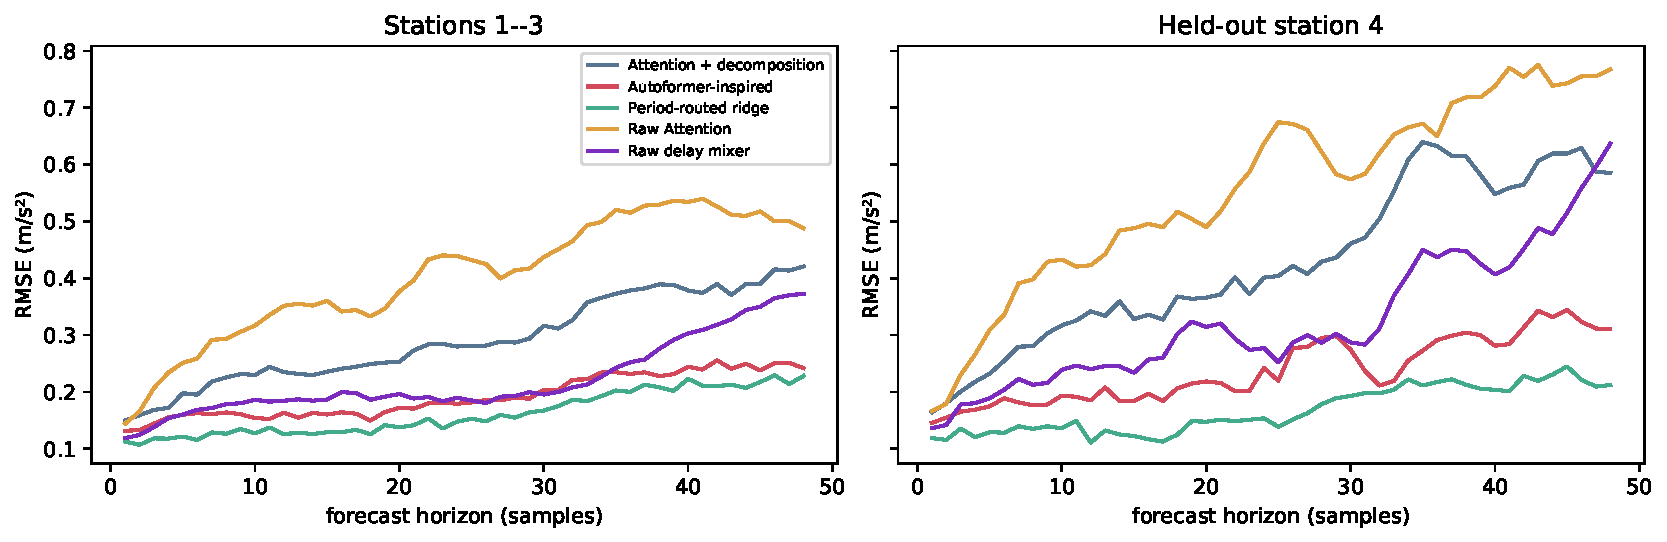
\includegraphics[width=.8\linewidth]{4.2-1.pdf}
\caption{Output 4.2: validation RMSE by forecast step.}
\end{figure}

\textbf{(c) Deployment choices.} \todo{confirm your choices; the draft below assumes
period-routed ridge for both, which is what the validation evidence favours. Keep $\le$200 words.}

\emph{Established stations: period-routed ridge.} It has the lowest validation RMSE (0.166 vs.\
0.196 for the best neural model, Autoformer-inspired) and the lowest MSE (0.028 vs.\ 0.038). It
uses 6$\times$ fewer parameters (59.9k vs.\ 373k) and fits in milliseconds instead of minutes. Its
error also grows the least with lead time.

\emph{Held-out Station 4: period-routed ridge.} Its advantage widens on the unseen station (0.173
vs.\ 0.245), because its conditioning variable, the estimated pace, is shared by all stations,
while the neural models partly fit station-specific patterns. Sensor-specific ridge cannot be used
here.

\emph{Answer to the central question.} In this world, the right inductive bias was worth more than
flexibility. A linear model told which variable matters beat every 370k-parameter network, and
among the networks the two structural switches mattered more than raw capacity. The caveat is that
the routed ridge depends on a hand-designed period estimator and pace bands that fit this
simulator exactly, and the Autoformer-inspired model is the strongest choice that does not need
that knowledge.

\textbf{Final test results (Output 4.3).} Both choices were entered before this cell was run.
\begin{center}\small
\begin{tabular}{llcccc}\toprule
Population & Model & Val.\ MSE & Val.\ RMSE & Test MSE & Test RMSE\\\midrule
Established (1--3) & Period-routed ridge & 0.0275 & 0.166 & 0.0260 & 0.161\\
Held-out Station 4 & Period-routed ridge & 0.0298 & 0.173 & 0.0333 & 0.183\\\bottomrule
\end{tabular}\end{center}
The test errors stay within about 6\% of validation for both populations, so the validation-based
choice held up on unseen data.

%=====================================================================
\section*{Task 2 -- Leaderboard Challenge}

\noindent Code: \texttt{Question 2 - Leaderboard/} (\texttt{autoformer.py}, \texttt{pipeline.py},
\texttt{eda\_figure.py}). Every number below is reproducible with the command given next to it.

%---------------------------------------------------------------------
\subsection*{2.1 What the data look like}

\begin{figure}[h]\centering
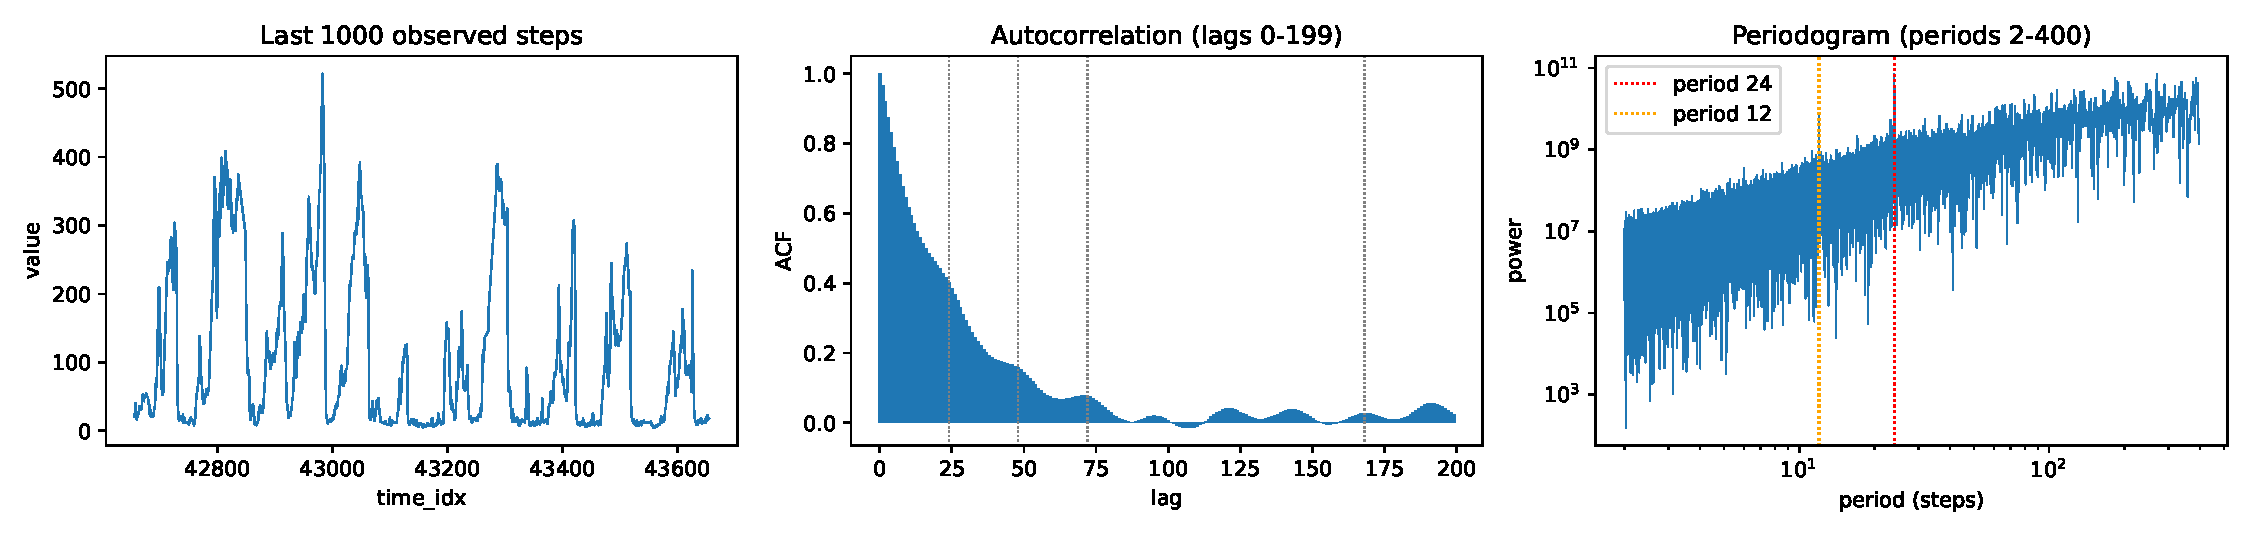
\includegraphics[width=\linewidth]{t2_eda.pdf}
\caption{Training target: last 1000 steps, ACF, and periodogram.}
\end{figure}

\begin{itemize}
  \item \textbf{Episodic and heavy-tailed.} The median is 73, the 99th percentile 418 and the max
  994. The series rises in multi-day episodes and then collapses abruptly. The periodogram is
  ``red'', with power rising towards long periods, so most of the variance is aperiodic episode
  structure rather than a cycle.
  \item \textbf{Short memory.} The ACF is 0.97 at lag 1, 0.57 at 12, 0.40 at 24, 0.16 at 48 and
  about 0.02 by 96. Beyond roughly two days the target's own history says little about the future.
  At $H{=}168$ most of the horizon is therefore beyond the target's own memory.
  \item \textbf{Recovered period.} With no timestamps, the periodogram shows clear peaks at
  \textbf{24} and its harmonic \textbf{12}, and the ACF has small bumps at 24, 48 and 72. I treat
  one step as one hour with a daily cycle and encode the phase $(\texttt{time\_idx} \bmod 24)$ as
  $\sin/\cos$ covariates. This is the only structure derived from the index. The ACF at 168 is
  0.03, so a weekly cycle is not used.
  \item \textbf{External file.} It has six continuous features (A--F) and four mutually exclusive
  binaries (G--J; exactly one is active at each step). Both are consistent with meteorological
  measurements, e.g.\ a categorical wind direction. Feature D (correlation $-0.35$ with
  $\log(1{+}y)$) and indicator H ($-0.35$; mean target 70 when active vs.\ 125 for J) are the most
  informative, so the covariates plausibly drive the \emph{onset and clearing} of episodes.
\end{itemize}

%---------------------------------------------------------------------
\subsection*{2.2 Validation protocol}

\begin{itemize}
  \item \textbf{Chronological split.} Training targets lie strictly before step 39{,}120. The
  validation targets are the final 4{,}536 observed steps (about 6 months), so validation sits
  directly before the hidden block, which follows step 43{,}656.
  \item \textbf{Many blocks, not one.} Validation forecast origins are every 24 steps, giving
  \textbf{183 overlapping 168-step forecasts}. I report pooled RMSE, MAE and sMAPE, plus the mean
  per-block RMSE. A single 168-step leaderboard score is one draw from that block-to-block
  distribution, so it is used only as confirmation.
  \item \textbf{Leakage control.} Target and covariate scalers (mean/std, with $\log1p$ applied to
  the skewed cumulative features D, E and F) are fitted on the training region only.
  \item \textbf{Seeds.} Every configuration is run with seeds $\{0,1,2\}$ and reported as mean
  $\pm$ std. A difference counts only if it clearly exceeds the seed spread.
  \item \textbf{Baselines} on the same 183 blocks (RMSE): training mean \textbf{87.8}, mean of last
  7 days 94.8, seasonal-naive (24) 117.9, persistence 122.2. The training mean beats persistence
  because 168 steps is well beyond the ACF memory, which shows how hard this horizon is.
\end{itemize}

%---------------------------------------------------------------------
\subsection*{2.3 Model}

Autoformer, written from scratch following Wu et al.\ (2021) \S\S3.1--3.2 and the structure of
the authors' reference implementation (\url{https://github.com/thuml/Autoformer}). Both
mechanisms required by \S2.4 are present:
\begin{itemize}
  \item \textbf{Series decomposition}: a centered moving average (kernel 25, about one daily cycle,
  with replicate padding) is applied to the input and inside \emph{every} encoder layer
  (2$\times$) and decoder layer (3$\times$). The decoder accumulates the extracted trend parts
  through a projection into the trend stream, which is initialised with the input's trend and the
  input mean.
  \item \textbf{Auto-Correlation} in place of dot-product attention: FFT-based delay scores
  $R(\tau)=\sum_t q_t k_{t-\tau}$, top-$k$ delays with $k=\lfloor \ln L\rfloor$ (factor $c{=}1$),
  softmax weights, and per-example time-delay aggregation of $v_{t-\tau}$. This is the same
  convention as my Task 1 \texttt{aggregate\_delays}. The reference code shares delays across the
  batch during training and reads $v_{t+\tau}$; I keep the Task 1 convention so that the value
  read back comes from the key position that scored.
  \item \textbf{Inputs.} The encoder sees $L$ past target values plus, at every step, the
  covariates (external features and daily phase) through a linear ``mark'' embedding. The decoder
  receives the last 48 steps' seasonal part plus zeros for the 168 future steps, and \emph{the
  covariates over the label and forecast window}. This is where future-known information enters an
  encoder--decoder model.
  \item \textbf{Size.} $d_\text{model}{=}32$, 4 heads, $d_\text{ff}{=}64$, 1 encoder and 1 decoder
  layer, giving about 22k trainable parameters. The leaderboard penalises parameters, so I started
  small and would grow the model only if validation justified it.
  \item \textbf{Training.} MSE on the standardised target (it matches the RMSE ranking metric),
  AdamW (lr $10^{-3}$, weight decay $10^{-4}$), batch 64, gradient clipping at 1, and every 4th
  training window per epoch. Early stopping uses validation RMSE with patience 2.
\end{itemize}

%---------------------------------------------------------------------
\subsection*{2.4 Does the external file help? (required ablation)}

The same model was trained in three modes, 3 seeds each, on the validation protocol above
(\texttt{python pipeline.py --exog \{none,past,full\}}):
\begin{center}\small
\begin{tabular}{lcccc}\toprule
External data used & RMSE & MAE & sMAPE & Block RMSE\\\midrule
None (target + daily phase only)               & 89.64 $\pm$ 0.74 & 69.1 $\pm$ 1.2 & 79.5 $\pm$ 0.3 & 81.8\\
Past only (up to the forecast origin)          & 88.91 $\pm$ 0.44 & 69.3 $\pm$ 1.3 & 79.5 $\pm$ 0.5 & 81.7\\
\textbf{Past + future (across the horizon)}    & \textbf{71.13 $\pm$ 1.46} & \textbf{55.9 $\pm$ 2.9} & \textbf{70.9 $\pm$ 1.6} & \textbf{67.3}\\
\midrule
\emph{Training-mean baseline} & 87.8 & 67.9 & 79.4 & 80.9\\\bottomrule
\end{tabular}\end{center}
\begin{itemize}
  \item \textbf{Clear positive result, but only for the future part.} Feeding the covariates over
  the forecast window lowers RMSE by 18.5 (about 21\%), which is more than 10 seed standard
  deviations. Past-only covariates change RMSE by 0.7, which is within seed noise.
  \item \textbf{Why the portion matters.} The ACF shows that the target forgets its past within
  about 2--4 days, and past covariates carry largely the same information as the past target. What
  decides the next week is \emph{when episodes start and clear}, and that is driven by conditions
  during the horizon itself (e.g.\ a change in the categorical regime G--J or a jump in D).
  So the covariates belong in the \emph{decoder}, aligned with the forecast steps; putting them
  only in the encoder wastes them.
  \item \textbf{Without them the Autoformer cannot beat the training mean} (89.6 vs.\ 87.8). This
  is an honest negative: at $H{=}168$ on a short-memory series, the target's own history alone
  adds nothing over the mean.
  \item \textbf{Metric disagreement.} With future covariates, sMAPE improves by 11\% but RMSE by
  21\%. The gain is concentrated on large values (episode peaks and clearings), which dominate the
  squared error. sMAPE is driven by low-level periods, where relative errors stay large.
\end{itemize}

%---------------------------------------------------------------------
\subsection*{2.5 Tuning}
Each variant changes \emph{one} setting of the past+future reference (the ablation's best row),
3 seeds, same validation protocol. Logs are in \texttt{results/tune.log}.
\begin{center}\small
\begin{tabular}{lccccc}\toprule
Variant & RMSE & MAE & sMAPE & Params & Epochs run\\\midrule
Reference ($L{=}336$, $d{=}32$, lr $10^{-3}$, raw target) & 71.13 $\pm$ 1.46 & 55.9 & 70.9 & 22{,}081 & 3.0\\
\textbf{$\log1p$ target} & \textbf{66.80 $\pm$ 0.89} & \textbf{44.1} & \textbf{54.5} & 22{,}081 & 5.7\\
lr $3{\times}10^{-4}$     & 67.60 $\pm$ 1.85 & 51.5 & 67.5 & 22{,}081 & 6.0\\
$d{=}16$, $d_\text{ff}{=}32$ & 67.89 $\pm$ 2.36 & 51.6 & 68.4 & $\approx$5.9k & 4.3\\
Huber loss                & 69.92 $\pm$ 2.07 & 53.1 & 68.5 & 22{,}081 & 3.0\\
drop feature C            & 70.17 $\pm$ 0.66 & 55.5 & 70.5 & 22{,}049 & 3.7\\
$L{=}168$                 & 70.20 $\pm$ 6.44 & 53.7 & 69.9 & 22{,}081 & 3.3\\
dropout 0.3, lr $3{\times}10^{-4}$ & 71.01 $\pm$ 0.89 & 55.6 & 70.1 & 22{,}081 & 4.7\\
$L{=}96$                  & 76.25 $\pm$ 3.70 & 57.4 & 73.3 & 22{,}081 & 3.3\\\midrule
log + lr $3{\times}10^{-4}$ + $d{=}16$ & 68.54 $\pm$ 1.30 & 44.6 & 54.8 & 5{,}921 & 10 (cap)\\
log + $d{=}16$            & 67.41 $\pm$ 2.96 & 43.7 & 54.1 & 5{,}921 & 8.0\\\bottomrule
\end{tabular}\end{center}
\begin{itemize}
  \item \textbf{The $\log1p$ target is the largest and most reliable gain:} RMSE $-4.3$, MAE
  $-21\%$, sMAPE $-23\%$, with the \emph{smallest} seed spread. The heavy right tail makes MSE on
  the raw scale dominated by a few peaks. The log scale lets the model learn the bulk of the
  distribution and the timing of episodes.
  \item \textbf{Long context matters.} $L{=}96$ is clearly worse and $L{=}168$ is unstable. The
  336-step window covers enough history for the decomposition and the delay scores to see several
  daily cycles and the preceding episode.
  \item \textbf{The gains did not stack.} Combining the log target with the lower learning rate
  and the smaller width was \emph{worse} than the log target alone. The small models were still
  improving at the 10-epoch cap or stalled early on some seeds ($\pm$2.96), so their parameter
  saving would be paid back in epochs and in unpredictability.
  \item \textbf{Metric disagreement.} The log target improves MAE and sMAPE far more than RMSE. It
  optimises something close to a \emph{geometric} mean, which is good on typical levels and biased
  low on spikes, and RMSE is the metric most sensitive to spikes.
\end{itemize}

%---------------------------------------------------------------------
\subsection*{2.6 Final submission and what the leaderboard taught me}
\textbf{Attempt \#1: a single refit model.}
\begin{itemize}
  \item \textbf{Model:} the $\log1p$-target configuration, seed 0. Early stopping on validation
  ran 7 epochs (best epoch 5; val RMSE 67.46). It was then refit on the full history for 5 epochs.
  $P=22{,}081$, $E=7+5=12$.
  \item \textbf{Leaderboard:} RMSE \textbf{142.04}, MAE 96.4, sMAPE 99.3\%, score 142.04. This
  is around the 97th percentile of the validation per-block RMSE (median 49), and the near-100\%
  sMAPE shows the forecast was far too low. The model had predicted a ``clean'' week (median 23.6),
  which the horizon covariates seemed to support.
\end{itemize}

\textbf{Diagnosis (training and validation data only; \texttt{diagnose*.py}).} A score in the tail
can be bad luck, so before using another attempt I checked whether the \emph{method} was fragile:
\begin{itemize}
  \item \textbf{The single-week forecast is unstable.} Across seeds 0--2, with and without refit,
  the forecast for the hidden week had means from \textbf{26 to 71}. The average pairwise RMSE
  between these six forecasts was 28.6. The submitted model was the lowest of the six.
  \item \textbf{The refit step was never validated.} For seed 0 it moved the forecast mean from 71
  (validated model) to 26. Pooled validation RMSE averages out such per-block variance; a single
  168-step block does not.
  \item \textbf{The log target is biased low in high weeks:} mean bias $-33.7$ on the top quartile
  of validation blocks by level.
\end{itemize}

\textbf{Attempt \#2: a 3-seed ensemble of validated models, no refit.} The decision rests on
validation:
\begin{center}\small
\begin{tabular}{lccccc}\toprule
 & Val RMSE & Val MAE & Block RMSE p90 & Block RMSE p97 & $P$ / $E$\\midrule
Single seeds 0/1/2 & 67.46 / 65.80 / 67.15 & 43.5--44.5 & 100--106 & 127--141 & 22{,}081 / 4--7\
\textbf{Mean of the 3 seeds} & \textbf{63.95} & \textbf{42.5} & \textbf{96} & \textbf{126} & 66{,}243 / 17\\bottomrule
\end{tabular}\end{center}
\begin{itemize}
  \item The ensemble beats every single seed on pooled RMSE and, above all, shortens the tail of
  bad blocks, which is where attempt \#1 landed.
  \item \textbf{Declared:} $\mathbf{P = 3\times22{,}081 = 66{,}243}$,
  $\mathbf{E = 7+6+4 = 17}$ (each member's early-stopping epochs; no refit).
  \item \textbf{Reproduce:} \texttt{python pipeline.py --final --exog full --target log --stride 4
  --max\_epochs 10 --patience 2 --seeds 0 1 2 --tag final\_ensemble}.
  \item \textbf{Leaderboard:} RMSE \textbf{112.15}, MAE 71.5, sMAPE 60.4\%, score \textbf{112.16}.
  That is 30 RMSE better than attempt \#1.
\end{itemize}

\textbf{Attempt \#3: log + raw ensemble, chosen on validation.} Attempt \#2 showed that the size
penalties are negligible, so larger ensembles cost almost nothing. I trained 5 log-target and 5
raw-target members with the same validated early stopping and no refit
(\texttt{ensemble\_members.py}). I then scored ensembles offline against attempt \#2 with a
paired bootstrap over weeks of validation blocks (\texttt{ensemble\_eval.py}). Neighbouring blocks
overlap, so the bootstrap resamples groups of 7 consecutive origins.
\begin{center}\small
\begin{tabular}{lcccccc}\toprule
Ensemble & Val RMSE & $\Delta$ vs \#2 [90\% CI] & Block p97 & Bias (top quartile) & $P$ & $E$\\\midrule
log $\times$3 (attempt \#2) & 63.95 & -- & 126 & $-36.8$ & 66{,}243 & 17\\
log $\times$5 & 63.39 & $-0.55$ [$-1.39$, $+0.22$] & 127 & $-38.8$ & 110{,}405 & 30\\
raw $\times$3 & 69.16 & $+5.21$ [$+1.31$, $+9.27$] & 114 & $-18.1$ & 66{,}243 & 9\\
raw $\times$5 & 67.66 & $+3.71$ [$-0.21$, $+7.97$] & 113 & $-13.5$ & 110{,}405 & 17\\
log $\times$5 + raw $\times$5 (equal) & 62.44 & $-1.51$ [$-3.65$, $+0.64$] & 117 & $-26.2$ & 220{,}810 & 47\\
\textbf{0.7 log $\times$5 + 0.3 raw $\times$5} & \textbf{62.05} & -- & -- & -- & 220{,}810 & 47\\\bottomrule
\end{tabular}\end{center}
\begin{itemize}
  \item \textbf{More log seeds alone barely help} ($-0.55$). Raw-target models alone are worse on
  RMSE and far worse on MAE and sMAPE, but they are much \emph{less biased on high-level weeks}
  ($-14$ to $-18$ vs.\ $-37$). The two errors are complementary, so mixing helps.
  \item \textbf{Mixing weight} (\texttt{ensemble\_weight.py}): for $\hat y=(1-w)\,\bar y_\text{log}
  + w\,\bar y_\text{raw}$, validation RMSE is flat for $w\in[0.2,0.5]$ and lowest at $w=0.3$
  (62.05). Re-choosing $w$ on 2000 bootstrap resamples picks 0.2--0.4 in 87\% of them and $w=0$
  (log only) in 0.2\%. A single scalar fitted on 183 blocks carries little overfitting risk, and
  $w=0.3$ beats the equal mix on RMSE, MAE and sMAPE.
  \item \textbf{Declared:} $P = 10\times22{,}081 = 220{,}810$; $E = 30 + 17 = 47$ (sum of each
  member's early-stopping epochs). Reproduce: \texttt{python ensemble\_members.py --targets log
  raw --seeds 0 1 2 3 4} then \texttt{python make\_submission.py --raw\_weight 0.3 --tag mix\_w03}.
  Rebuilding the log $\times$3 ensemble from the saved members reproduces attempt \#2 exactly.
  \item \textbf{Leaderboard:} RMSE \textbf{102.21}, MAE 64.5, sMAPE 56.5\%, score
  \textbf{102.23}. This is the submission the leaderboard uses.
  \item \textbf{Caveat:} the gain on validation was about 1.9 RMSE, and the confidence interval of
  the closely related equal mix included zero. The 10-point leaderboard gain is therefore partly
  luck on one week. The raw members also forecast a higher week, which attempt \#1 had already
  suggested was the truth. I chose the candidate and its weight on validation only, but attempt
  \#1's result is what motivated spending another attempt.
\end{itemize}

\textbf{Lessons.}
\begin{itemize}
  \item \textbf{Size penalties are tiny here.} Score $-$ RMSE was 0.006, 0.009 and 0.024 for
  attempts \#1--\#3 ($P$ from 22k to 221k). Differences between designs are tens of RMSE points,
  so on this leaderboard variance reduction is worth far more than parameter economy.
  \item \textbf{A good pooled validation score does not guarantee a good single-block score.}
  I should have checked the stability of the forecast at the actual forecast origin before the
  first submission, and not shipped an unvalidated refit.
  \item \textbf{Transparency.} Leaderboard results \emph{prompted} the diagnosis and the decision to
  use more attempts. Each submitted candidate and its settings were chosen on the validation
  evidence above; no setting was tuned to the leaderboard score. Two of the five attempts were left
  unused.
\end{itemize}

%---------------------------------------------------------------------
\subsection*{2.7 Limitations}
\begin{itemize}
  \item The validation period (the last 6 months) is a single stretch of the series. If the
  hidden block's behaviour differs from it, the validation ranking may not carry over.
  \item The model treats the future covariates as given; their own measurement noise is not
  modelled.
  \item The daily phase assumes the period-24 cycle seen in the training spectrum continues into
  the horizon.
\end{itemize}

%---------------------------------------------------------------------
\subsection*{2.8 Reflection questions}

\textbf{Q2.1 -- Auto-Correlation vs.\ self-attention.}
\begin{itemize}
  \item \emph{Where Auto-Correlation is strictly better:} stationary signals made of a few stable
  periods, where every pair $(t,t-P)$ is related for the same reason. Tying all such pairs into
  one score $R(P)$ pools evidence over the whole window, at $O(L\log L)$ cost. Attention must
  rediscover the same relation pair by pair, at $O(L^2)$, with more variance. Task 1 is an
  example: delay mixing alone cut MSE by 70\% vs.\ 47\% for decomposition.
  \item \emph{What it throws away:} anything that is not a series-level shift. That includes
  content-specific, non-stationary links between \emph{individual} positions, e.g.\ ``the value
  right after the last regime change'' or a single precursor event. Its aggregation copies whole
  shifted sequences, so position-specific relevance is lost. On our Task 2 series, whose spectrum
  is red and episodic, there is little periodic structure for it to exploit. This is one reason the
  model without covariates did not beat the mean.
  \item \emph{When the period drifts over time:} within one window, no single lag aligns the
  whole sequence. The peaks of $R(\tau)$ broaden and lower, and the aggregated copies go out of
  phase (destructive averaging). Attention degrades more gracefully, because each query can pick
  its own key, but it still has to learn the drift from data.
\end{itemize}

\textbf{Q2.2 -- What the moving-average trend assumes.}
\begin{itemize}
  \item It assumes the trend is \emph{locally linear over the kernel} and much slower than the
  seasonality. Only then does averaging remove the cycle and keep the trend.
  \item \emph{Boundaries:} replicate padding biases the last $k/2$ trend values towards the end
  value. The trend flattens exactly at the forecast origin, which is the most important point.
  (Task 1, Output 2.1 shows this right-edge flattening.)
  \item \emph{Curvature:} the filter is exact for linear trends only. At a peak of a curved
  trend it under-shoots, and the curvature leaks into the seasonal part.
  \item \emph{Abrupt level shift:} the shift is smeared into a ramp of width $k$, and an
  S-shaped artefact appears in the seasonal component on both sides of it.
  \item \emph{Alternative:} STL (LOESS-based) or a learnable/robust trend (e.g.\ median filter, or
  a Hodrick--Prescott-style penalised fit). STL buys adaptivity to curvature and robustness to
  outliers, under the assumption that the trend is \emph{smooth but not necessarily linear}. It
  gives up a single fixed kernel, adds hyperparameters, costs more, and is not a simple
  differentiable layer to apply in every block. A median filter preserves level shifts but is
  non-smooth.
\end{itemize}

\textbf{Q2.3 -- Progressive vs.\ one-shot decomposition.}
\begin{itemize}
  \item \emph{What it buys:} each block's mixing and feed-forward layers create new
  low-frequency content in the \emph{learned} representation, e.g.\ residual connections
  re-adding slow structure. Interleaved decomposition removes it again before the next mixer, so
  every Auto-Correlation sees a near-zero-mean seasonal stream. A one-shot preprocessing step
  works only on the raw input and cannot do this. The decoder can also refine the trend
  progressively by accumulating each layer's extracted trend.
  \item \emph{When it hurts:} when the useful ``seasonal'' signal is itself slower than the
  kernel. Take a weekly cycle with $k=25$ on hourly data: every block pushes more of that cycle
  into the trend path, which is only a linear projection and cannot model it. The mixer never sees
  it. Repeatedly applying the same low-pass filter also compounds the boundary bias at every layer.
\end{itemize}

\textbf{Q2.4 -- $k = c\log L$.}
\begin{itemize}
  \item \emph{Larger $k$:} more lags are blended. This hedges under uncertainty (the Task 1
  argument about squared error), but it averages in weak or spurious lags, which blurs sharp
  periodic structure. Compute also grows.
  \item \emph{Smaller $k$:} the model commits to the strongest lag. That is sharp if the lag is
  right and costly if it is wrong. It also cannot represent several co-existing periods.
  \item \emph{Principled or convenient?} Mostly convenient. It keeps the total cost at
  $O(L\log L)$, matching the FFT, and it grows slowly because longer windows contain more harmonics
  of the same periods. No statistical argument fixes $\log L$ as the right count.
  \item \emph{The better rule:} $k$ should be about the number of distinct periodicities times
  the harmonics/multiples worth keeping, e.g.\ for Task 2 the lags 24 and 12 and their multiples.
  Ideally it would be chosen from the significance of the peaks in $R(\tau)$, not from $L$.
\end{itemize}

\textbf{Q2.5 -- One-shot vs.\ autoregressive horizons.}
\begin{itemize}
  \item \emph{Error accumulation and exposure bias:} the autoregressive approach is trained on true
  inputs but fed its own predictions at test time. Errors therefore compound, and the inputs come
  from a distribution never seen in training. One-shot (direct) forecasting, as in Autoformer,
  avoids both.
  \item \emph{Error correlation:} autoregressive errors are strongly positively correlated along
  the horizon, because one early miss shifts everything after it. Direct-forecast errors at
  different steps are less coupled, but the forecast can be less self-consistent, e.g.\ jagged or
  smoothed towards the mean, as our model does beyond the ACF memory.
  \item \emph{When each is preferable:} autoregressive suits low-noise, near-deterministic
  dynamics with short horizons (e.g.\ a well-identified AR process), where re-using the transition
  model is efficient. Direct suits noisy, heavy-tailed series and long horizons. The longer the
  horizon, the more the comparison favours direct (or hybrid, e.g.\ multi-step blocks) methods.
\end{itemize}

\textbf{Q2.6 -- Window-relative normalisation (RevIN-style).}
\begin{itemize}
  \item \emph{What is destroyed:} the absolute level and scale of the window, i.e.\ where the
  series sits relative to its long-run distribution.
  \item \emph{When that matters:} when the future depends on the absolute level, e.g.\
  mean-reversion towards a global mean, physical bounds (non-negativity, saturation), or regimes
  defined by level (a pollution episode at 400 behaves differently from a calm period at 20).
  \item \emph{Helps a lot:} a series with drifting level/scale but stable shape, e.g.\ sales
  growing over years with the same weekly pattern. Without it, the model would extrapolate outside
  the training range.
  \item \emph{Provably loses something:} a mean-reverting series such as an OU process. Two
  windows with identical shape at levels $+3\sigma$ and $-3\sigma$ need opposite forecasts (one
  falls, one rises). After normalisation they are identical inputs, so no model can separate them,
  unless the statistics are fed back in as features. Our Task 2 series is of this kind: at
  $H{=}168$ the best naive forecast is the \emph{global} mean (87.8), not the window mean (94.8).
  That is why I used global, training-fitted scaling.
\end{itemize}

\textbf{Q2.7 -- Past-known vs.\ future-known covariates.}
\begin{itemize}
  \item The distinction changes \emph{where} they enter, not just how much they help.
  Past-only covariates belong in the encoder, alongside the target history. Future-known
  covariates must also reach the \emph{decoder}, aligned with the forecast steps, so that step
  $t{+}h$ can condition on $x_{t+h}$. Putting a future-known variable only in the encoder throws
  away exactly its useful part.
  \item \emph{Informative only when future-known:} a fast-acting exogenous driver with little
  persistence, e.g.\ wind or rain in the hour being forecast (for pollution), or a scheduled
  promotion (for sales). Its past values say little about $y_{t+h}$. Our ablation shows exactly
  this: past only gives 88.9 ($\approx$ none, 89.6); past+future gives 71.1.
  \item \emph{Equally useful in both:} a slowly varying or deterministic covariate whose past
  determines its future, e.g.\ a daily-phase indicator, a holiday calendar, or a slowly drifting
  temperature trend. Knowing its future adds nothing to knowing its past.
\end{itemize}

\textbf{Q2.8 -- No calendar features.}
\begin{itemize}
  \item \emph{What is lost:} hour-of-day, day-of-week and month/season effects, as well as holidays
  and irregular calendar events (moving holidays, DST shifts). The model also cannot align
  multi-scale cycles without being told the base unit.
  \item \emph{How to recover it:} periodogram/ACF peaks (here 24 and 12, so a daily cycle in
  hourly data), then phase features $\sin/\cos(2\pi\,\texttt{idx}/P)$. Auto-Correlation also
  discovers dominant lags implicitly.
  \item \emph{What must hold for this to be trustworthy:} the sampling is truly uniform with no
  gaps (guaranteed here), the period is stationary over the training span and the horizon, and
  the peak is genuinely significant, not a leakage artefact of a red spectrum. It should be
  checked on separate sub-periods. Holidays and other irregular events cannot be recovered this way.
\end{itemize}

\textbf{Q2.9 -- Structural models vs.\ decomposition Transformers.}
\begin{itemize}
  \item \emph{Structural models (ETS/SARIMA/state-space) win} with short series (hundreds to a few
  thousand points), low signal-to-noise, and a regular, stable seasonal structure. Their strong
  priors are roughly correct and their few parameters keep variance low.
  \item \emph{Transformers win} with long series (tens of thousands of points or many related
  series), rich covariates, non-linear interactions, and several or varying seasonalities that
  linear structural forms cannot express. Here the extra parameters are paid for by data.
  \item \emph{Deciding beforehand:} compare the length to the parameter count (here 43k points vs.\
  about 22k parameters, which is borderline). Check the spectrum's regularity: a few sharp peaks
  favour structural models; a red, episodic spectrum favours flexible ones. Fit a cheap structural
  baseline and a linear model with covariates first, and accept the Transformer only if it beats
  them on rolling-origin validation by more than the seed spread. In our case the
  Transformer without covariates did not beat the training mean, while with future covariates it
  did by a wide margin. So any advantage comes from \emph{using covariates}, not from the target's
  own dynamics. A linear model with covariates would be the right next baseline to test whether
  that advantage needs the Transformer at all.
\end{itemize}

%=====================================================================
\section*{Use of generative AI}
\todo{Required by the course policy: list the prompts used, a summary of the outputs (code
stubs, Task 2 pipeline, draft report text), and the edits you made.}

\end{document}
